\documentclass[discrete.tex]{subfiles}

\begin{document}
  \section{Метод Барроуза-Уилера}

  \begin{alg}
      \begin{enumerate}
          \item Составляется таблица всех циклических сдвигов строки.
          \item Производится лексикографическая сортировка строк таблицы.
          \item В качестве выходной строки выбирается последний столбец таблицы преобразования и номер строки, совпадающей с исходной.
      \end{enumerate}
  \end{alg}

  \begin{Example}
      \[
      \begin{tabular}{c|c|c|c}
          \text{Вход} & \text{ц. сдвиги} & \text{сортировка} & \text{Выход}\\ \hline
          & \ul{abacaba} & aabacab & \\ \hline
          & bacabaa & abaabac &\\ \hline
          & acabaab & \ul{abacaba} & \\ \hline
          abacaba & cabaaba & acabaab & bcabaaa, 3\\ \hline
                  & abaabac & baabaca &\\\hline
                  & baabaca & bacabaa &\\\hline
                  & aabacab & cabaaba &
      \end{tabular}
      \]
      BWT("abacaba") = ("bcabaaa"{}, 3)
  \end{Example}

  \begin{alg} [обратного преобразования]
      Пусть нам дали BWT(S) = (A, x)\\ Тогда выпишем в столбик A, отсортируем, слева допишем
      A, снова отсортируем, так n раз,  где n - длина строки A.
      После последней сортировки мы получим, что строка с номером x - S
  \end{alg}

  \begin{example}[по Григорьевой]
    $S_1=$РЕФРИЖЕРАТОР\$
    \begin{figure}[H]
        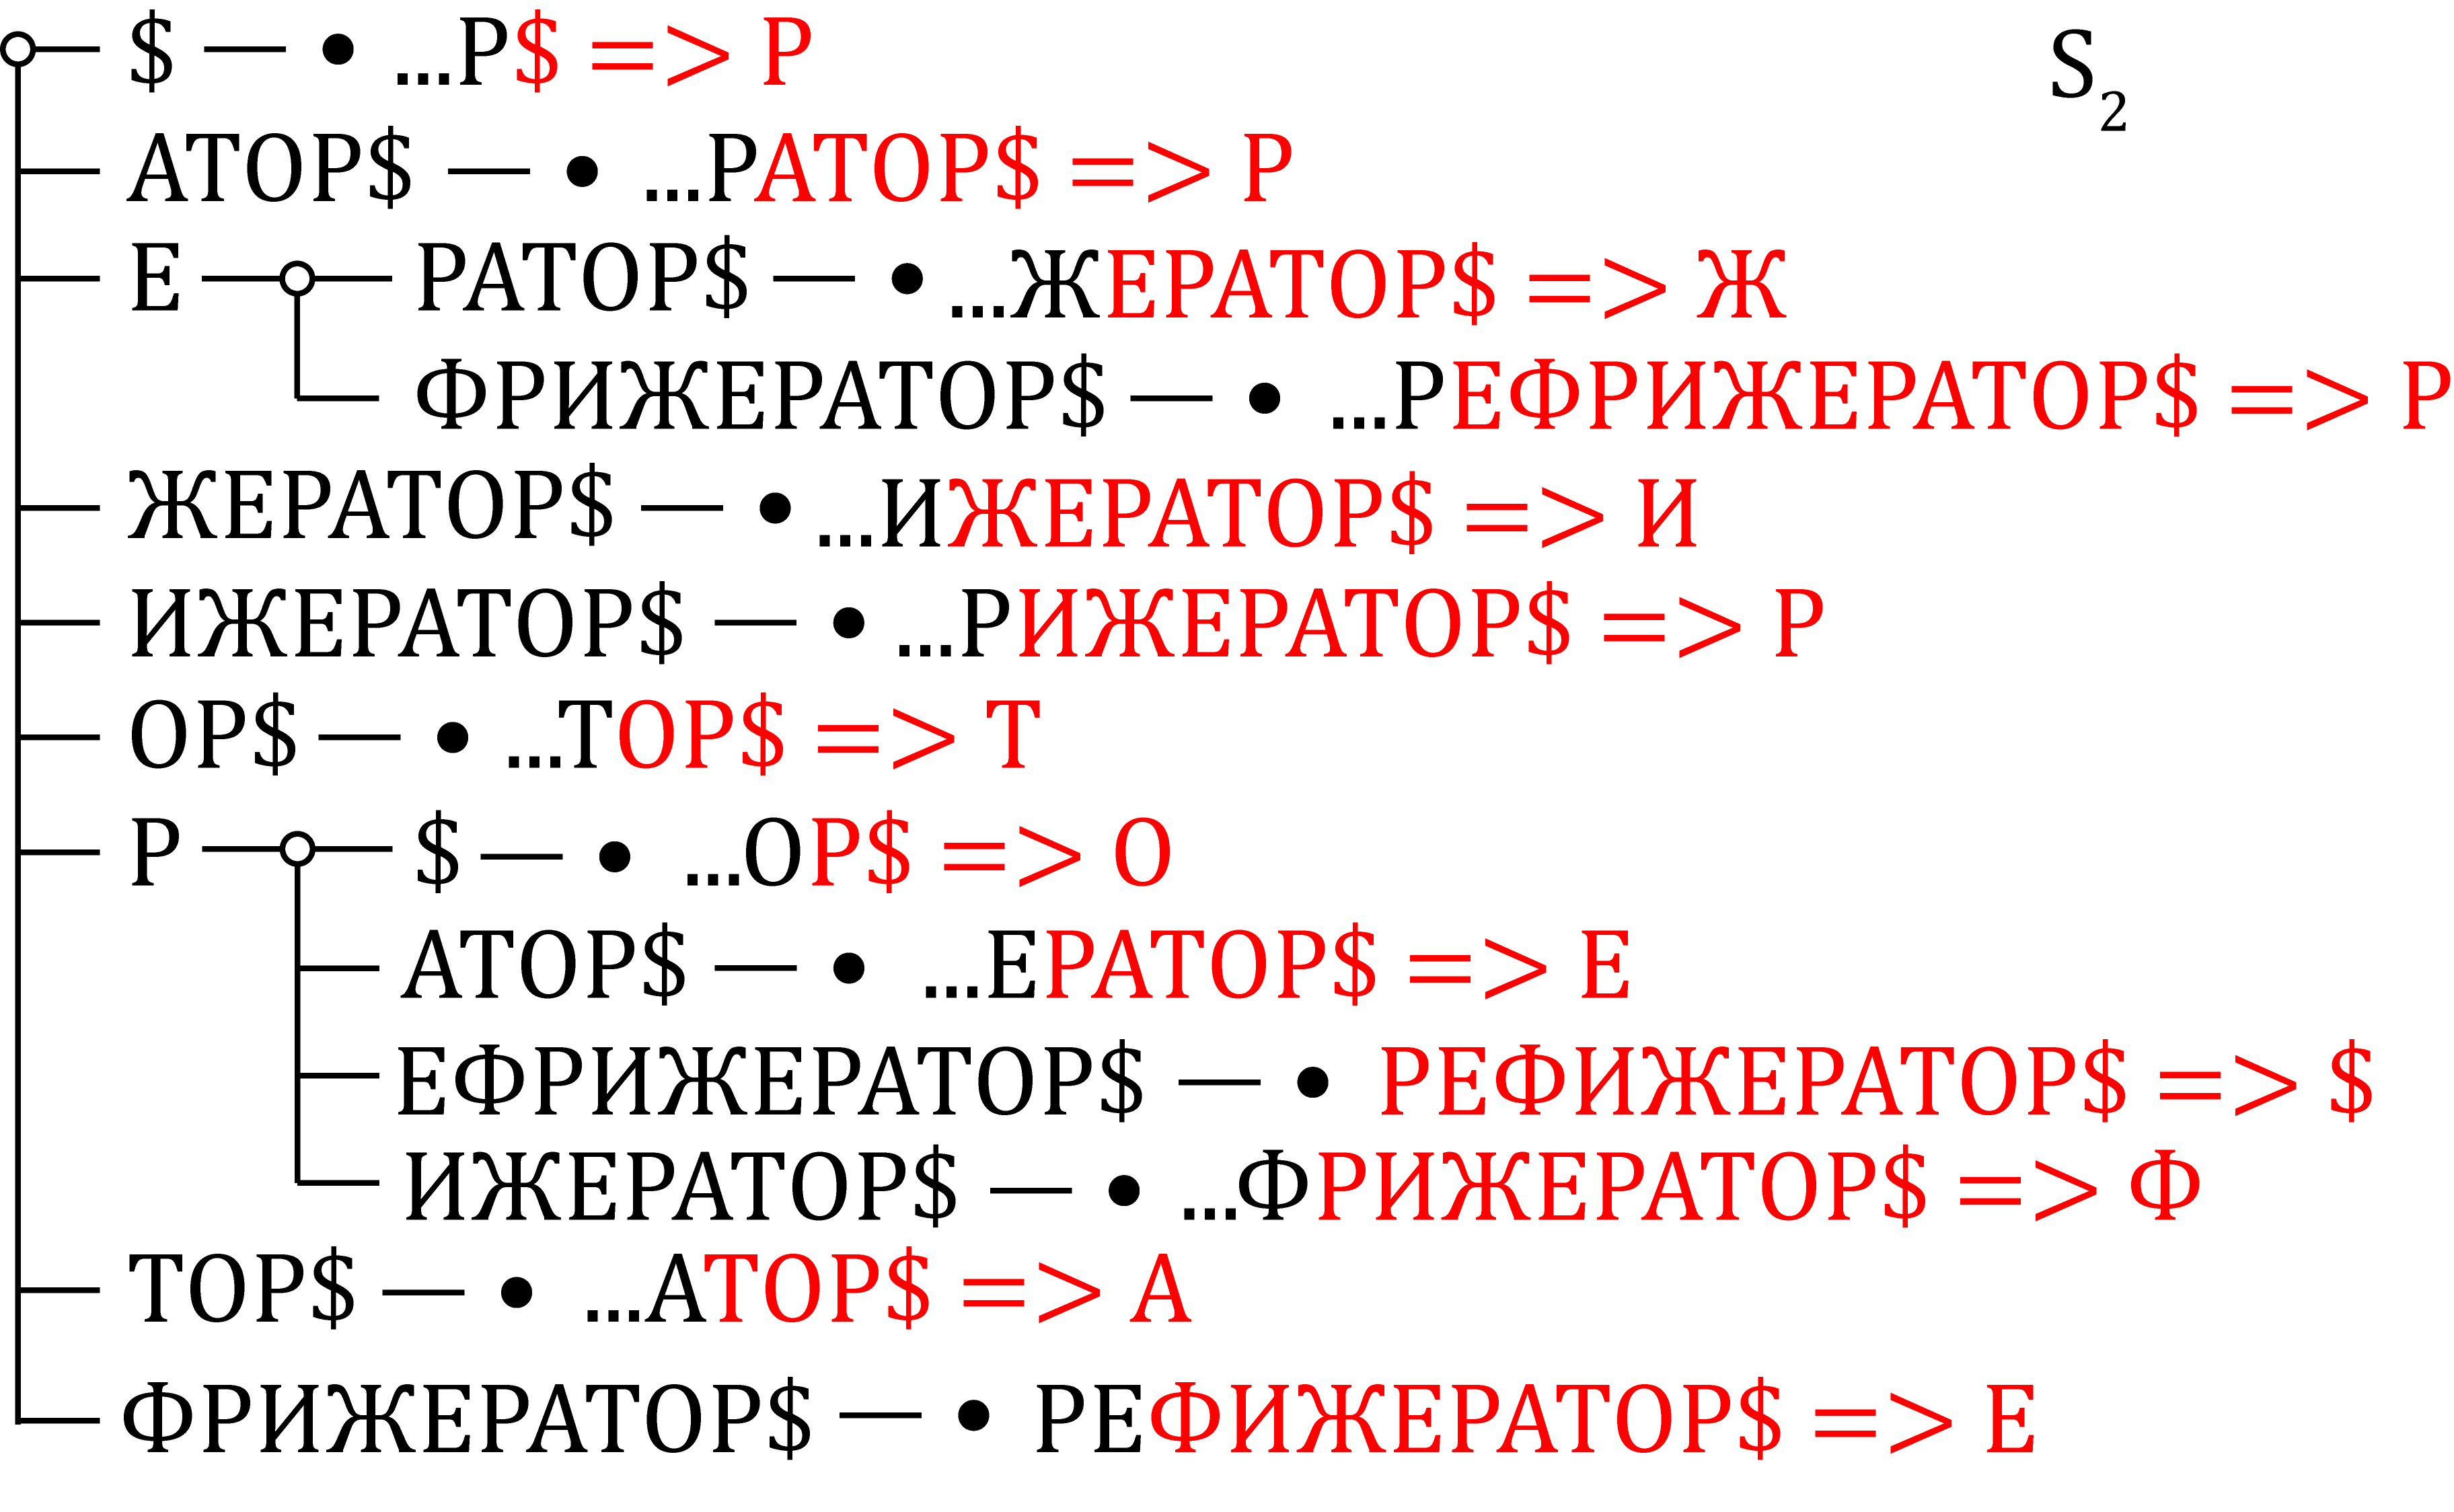
\includegraphics[height=5cm]{pics/27_1.png}
        \centering
    \end{figure}
    Чтобы получить $S_2$ берем первый символ, стоящий перед каждым последним суффиксом:\\
    $S_2=$РРЖРИРТОЕ\$ФАЕ\\ \ \\
    Теперь составим таблицу, в которой:\\
    1 столбец - строка $S_2$
    2 столбец - номер символа в 3 стобце предыдущей строки (если символа не было, то ставим 0)\\
    3 столбец - ставим символ на первую позицию и записываем оставшуюся часть строки\\
    \begin{tabular}{c|c|c}
      Р & 0 & Р\\
      Р & 1 & Р\\
      Ж & 0 & ЖР\\
      Р & 2 & РЖ\\
      И & 0 & ИРЖ\\
      Р & 2 & РИЖ\\
      Т & 0 & ТРИЖ\\
      О & 0 & ОТРИЖ\\
      Е & 0 & ЕОТРИЖ\\
      \$& 0 & \$ЕОТРИЖ\\
      Ф & 0 & Ф\$ЕОТРИЖ\\
      А & 0 & АФ\$ЕОТРИЖ\\
      Е & 4 & ЕАФ\$ОТРИЖ
    \end{tabular}
    Результат: ЕАФ\$ОТРИЖ + 0102020000004\\ \ \\
    Теперь попробуем декодировать *каким-то образом строим такую же табличку*\\
    ???
  \end{example}
\end{document}
